Find a subspace $X$ of $\mathbb{R}^2$ and an equivalence relation $\sim$ on $X$ so that
$X/\sim\cong S^2$, where $S^2$ is the unit sphere centered at the origin in $\mathbb{R}^3$.
Illustrate typical open sets in the quotient space and in $X$. You do not have to give an explicit
homeomorphism between $X/\sim$ and $S^2$, but you should describe a function between the two and explain
why it is a homeomorphism.\\\\

\begin{solution}\renewcommand{\qedsymbol}{}\ \\
    Consider the set $D=\{(x,y)\in\mathbb{R}^2|x^2+y^2\leq1\}$ and define $\sim$ by
    $(x_1,y_1)\sim(x_2,y_2)$ if $\sqrt{x_1^2+y_1^2}=\sqrt{x_2^2+y_2^2}=1$, and $(x,y)\sim(x,y)$
    otherwise. T0hen we have that $D/\sim\cong S^2$. The function that is a homeomorphism, $f$, takes
    each point on $D/\sim$ and maps it to a unique point on the unit sphere. $f$ also maps to every
    point on $S^2$. In particular, $f$ maps points in $D/\sim$ that are given by $x^2+y^2<1$ to some
    point on the surface of $S^2$ and the points given by $x^2+y^2=1$ are mapped to the 'pole' of $S^2$
    as shown below. For example, $(0,0)$ maps to the point $(0,0,-1)$ since each point on $S^2$ is a
    distance of one form $(0,0,0)$. Another example would be $(0,1)$ would map to $(0,0,1)$ by the same
    logic due to the equivalence relation. Also, the point $(0,\frac12)$ on the cicrle of radius
    $\frac12$ would map to $(0,\frac12,\sqrt{\frac34})$ so that the point is a distance of one away from
    the origin in $\mathbb{R}^3$. So, every concentric circle of radius $\epsilon<1$ would map to some
    circle on $S^2$ such that the $z$ coordinate would be $z^2=1-x_{\epsilon}^2-y_{\epsilon}^2$ where
    $x_{\epsilon},y_{\epsilon}$ are points on the circle of radius $\epsilon$. Now in particular, $f$
    maps open surface patches on $D/\sim$ to open patches on $S^2$. Similarly, $f^{-1}$ maps open
    patches on $S^2$ to open patches on $D/\sim$. Example open sets on both $D$ and $D/\sim$ are given
    below.
    
    \begin{center}
    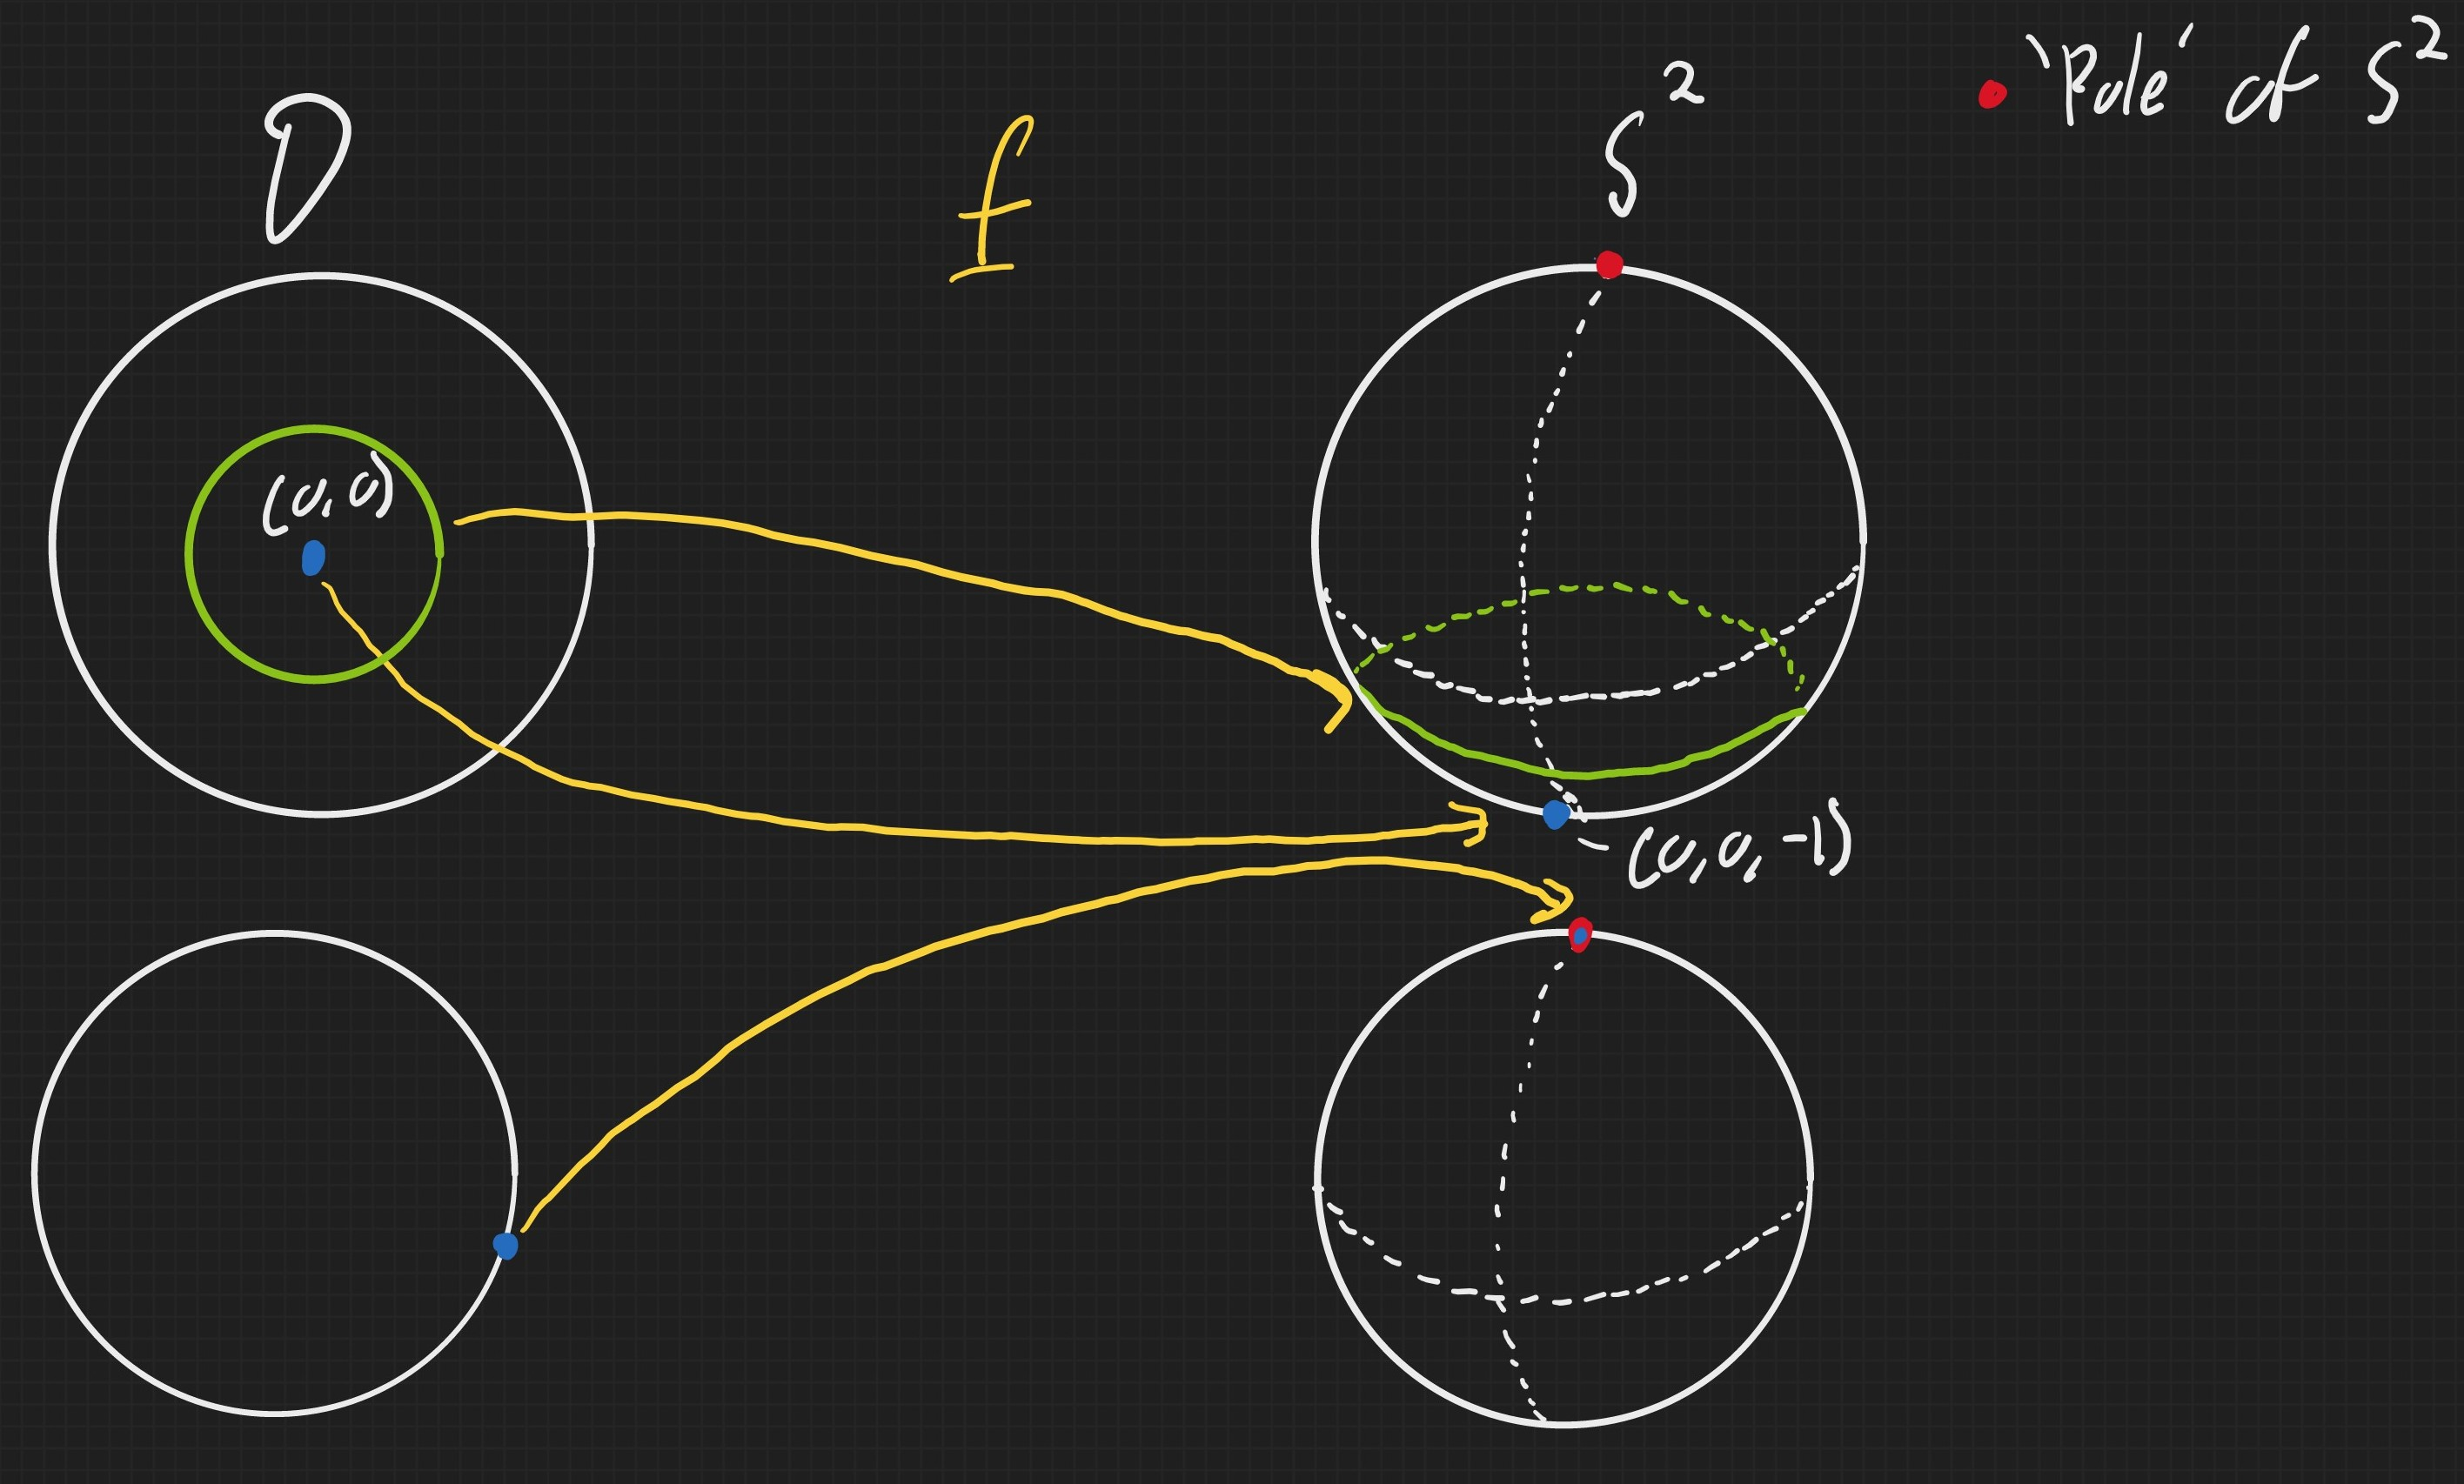
\includegraphics[scale=0.4]{ps7p222.JPG}
    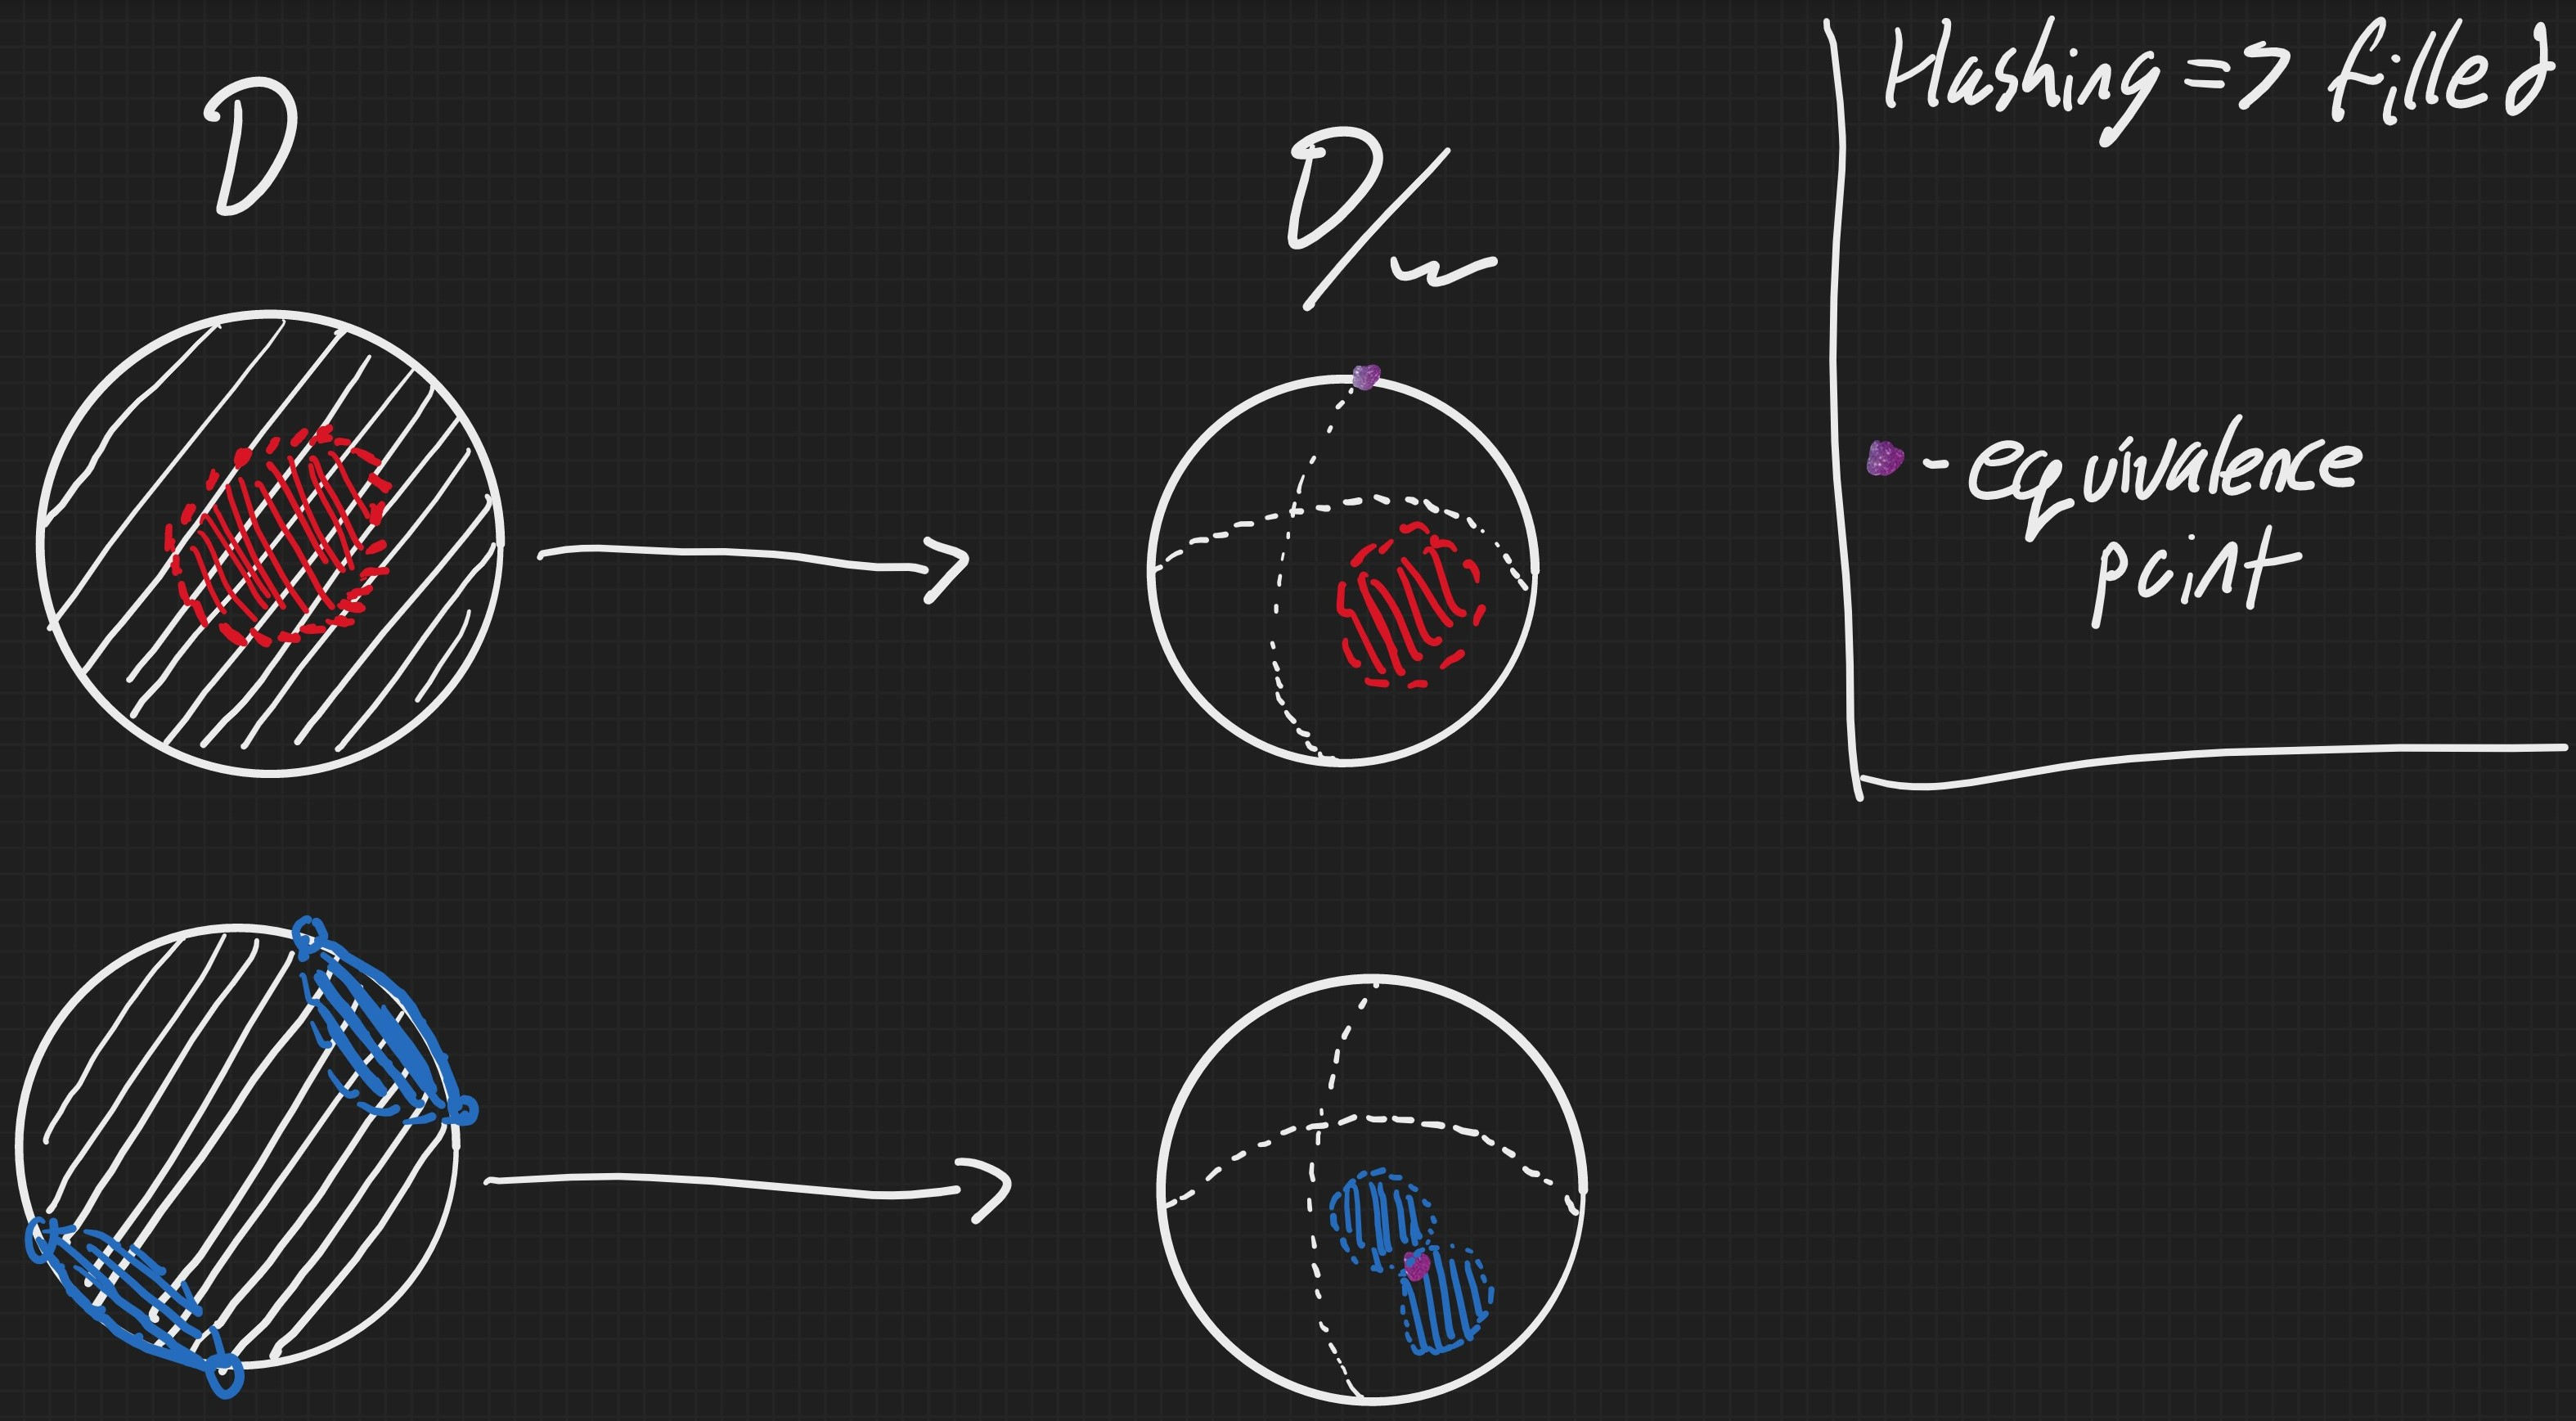
\includegraphics[scale=0.4]{ps7p2.JPG}
    \end{center}

\end{solution}